\documentclass[a4paper,10pt,ngerman]{scrartcl}
\usepackage{babel}
\usepackage[T1]{fontenc}
\usepackage[utf8x]{inputenc}
\usepackage[a4paper,margin=2.5cm,footskip=0.5cm]{geometry}

% Die nächsten drei Felder bitte anpassen:
\newcommand{\Aufgabe}{Aufgabe 1: \LaTeX-Dokument} % Aufgabennummer und Aufgabennamen angeben
\newcommand{\TeilnahmeId}{?????}                  % Teilnahme-ID angeben
\newcommand{\Name}{Vor- und Nachname}             % Name des Bearbeiter / der Bearbeiterin dieser Aufgabe angeben

% Kopf- und Fußzeilen
\usepackage{scrlayer-scrpage, lastpage}
\setkomafont{pageheadfoot}{\large\textrm}
\lohead{\Aufgabe}
\rohead{Teilnahme-ID: \TeilnahmeId}
\cfoot*{\thepage{}/\pageref{LastPage}}

% Position des Titels
\usepackage{titling}
\setlength{\droptitle}{-1.0cm}

% Für mathematische Befehle und Symbole
\usepackage{amsmath}
\usepackage{amssymb}

% Für Bilder
\usepackage{graphicx}

% Für Algorithmen
\usepackage{algpseudocode}
\usepackage{amsthm}
\usepackage{tabularx}
\usepackage{booktabs}

% Für Quelltext
\usepackage{listings}
\usepackage{color}
\definecolor{mygreen}{rgb}{0,0.6,0}
\definecolor{mygray}{rgb}{0.5,0.5,0.5}
\definecolor{mymauve}{rgb}{0.58,0,0.82}
\lstset{
  keywordstyle=\color{blue},commentstyle=\color{mygreen},
  stringstyle=\color{mymauve},rulecolor=\color{black},
  basicstyle=\footnotesize\ttfamily,numberstyle=\tiny\color{mygray},
  captionpos=b, % sets the caption-position to bottom
  keepspaces=true, % keeps spaces in text
  numbers=left, numbersep=5pt, showspaces=false,showstringspaces=true,
  showtabs=false, stepnumber=2, tabsize=2, title=\lstname
}
\lstdefinelanguage{JavaScript}{ % JavaScript ist als einzige Sprache noch nicht vordefiniert
  keywords={break, case, catch, continue, debugger, default, delete, do, else, finally, for, function, if, in, instanceof, new, return, switch, this, throw, try, typeof, var, void, while, with},
  morecomment=[l]{//},
  morecomment=[s]{/*}{*/},
  morestring=[b]',
  morestring=[b]",
  sensitive=true
}

% Diese beiden Pakete müssen zuletzt geladen werden
%\usepackage{hyperref} % Anklickbare Links im Dokument
\usepackage{cleveref}

% Daten für die Titelseite
\title{\textbf{\Huge\Aufgabe}}
\author{\LARGE Teilnahme-ID: \LARGE \TeilnahmeId \\\\
  \LARGE Bearbeiter/-in dieser Aufgabe: \\
  \LARGE \Name\\\\}
\date{\LARGE\today}
\newtheorem{theorem}{Satz}
\newtheorem{lemma}[theorem]{Lemma}
\begin{document}

\maketitle
\tableofcontents

\vspace{0.5cm}

\textbf{Anleitung:} Trage oben in den Zeilen 8 bis 10 die Aufgabennummer, die Teilnahme-ID und die/den Bearbeiterin/Bearbeiter dieser Aufgabe mit Vor- und Nachnamen ein.
Vergiss nicht, auch den Aufgabennamen anzupassen (statt "`\LaTeX-Dokument"')!

Dann kannst du dieses Dokument mit deiner \LaTeX-Umgebung übersetzen.

Die Texte, die hier bereits stehen, geben ein paar Hinweise zur Einsendung. Du
solltest sie aber in deiner Einsendung wieder entfernen!

\section{Lösungsidee}
\section{Beliebige Lösung}
\subsection{Einleitung}
\begin{figure}[t]
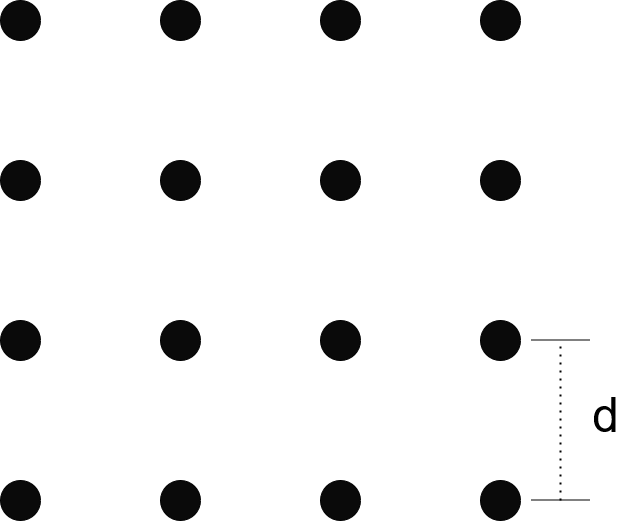
\includegraphics[scale=.2]{struktur}
\centering
\caption{Die 16-Struktur.}
\end{figure}
\begin{figure}[t]
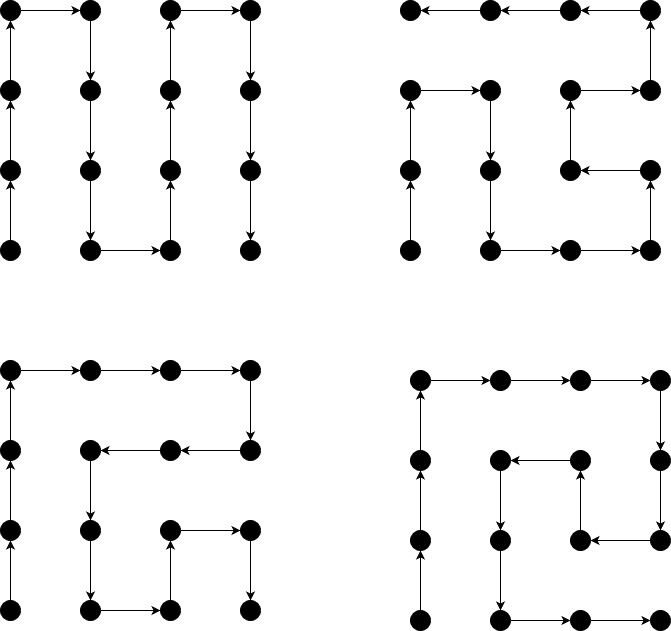
\includegraphics[scale=0.5]{richtungen}
\centering
\caption{Ein von unten in die 16-Struktur kommendes Flugzeug kann in alle Richtungen weiter fliegen. Für andere Herkunftsrichtungen müssen die Pfade entsprechend gedreht werden.}
\end{figure}
Es ist $\mathcal{NP}$-schwer, das weniger krumme Touren-Problem (WKT) optimal
zu lösen. Um das zu zeigen, wird eine Reduktion vom eulerschen Pfad-Problem des
Handlungsreisenden (E-PTSP) skizziert, welches bekanntermaßen
$\mathcal{NP}$-schwer ist. E-PTSP lautet folgendermaßen: Sei $P \subset
  \mathbb{R}^2$ eine endliche Menge. Dann wird eine Reihenfolge von P gesucht,
bei der die Strecke zwischen aufeinanderfolgenden Punkten minimal ist. \\
E-PTSP kann nun auf WKT reduziert werden, in dem jeder der Punkte $P$ durch
eine 16-Struktur ersetzt wird. Wie die Abbildung zeigt,
kann eine 16-Struktur aus beliebigen Richtungen angeflogen werden.\\
Diese Transformation heißt im folgenden $T_d: \mathfrak{P}(\mathbb{R}) \rightarrow \mathfrak{P}(\mathbb{R})$
 mit $d \in \mathbb{R}$,
wobei $\mathfrak{P}$ für die Potenzmenge steht.
\begin{lemma}
 Es sei $P \subset \mathbb{R}; |P| < \infty$ eine Instanz von E-PTSP. 
 $P' = T_d(P)$ kann in eine mögliche Lösung von $P$ umgewandelt werden,
 wenn die Punkte jeder 16-Struktur jeweils direkt nacheinander angeflogen werden.
\end{lemma}
\begin{proof}
 Jeder Punkt in $P'$ darf genau einmal besucht werden. Wenn die Punkte einer 16-Struktur
 direkt hintereinander angeflogen werden, kann diese Struktur danach nicht mehr angeflogen werden.
 Dadurch wird in einer solchen Lösung jede 16-Struktur nur einmal angeflogen. Die Lösung stellt also
 eine Permutation der 16-Strukturen dar. Da jede 16-Struktur einen entsprechenden Punkt in $P$ hat,
 kann die Permutation der 16-Strukturen so in eine Permutation von $P$ umgewandelt werden.
\end{proof}
Nun sei $\lim \limits_{d \to 0}$. Die Abstände zwischen Punkten gleicher 16-Strukturen
nähert sich dann $0$ an, während die Abstände zwischen Punkten unterschiedlicher 16-Strukturen den Abständen
der entsprechenden Punkte in der E-PTSP-Instanz annähern. Die Länge eines Pfades, der die Punkte einer
16-Struktur unmittelbar nacheinander besucht, nähert sich dann dem entsprechenen Pfad in der E-PTSP-Instanz an.
Es muss jetzt noch gezeigt werden, dass eine optimale Lösung die Punkte einer Struktur unmittelbar nacheinander
besucht und deshalb in eine Lösung des entsprechenden E-PTSP umgewandelt werden kann. Nach dem Beweis von
Lemma 1 ist das äquivalent mit der Aussage, dass eine optimale Lösung jede 16-Struktur nur einmal besucht.
\begin{lemma}
  Es sei $P$ eine Instanz von E-PTSP und $P'=T_d(P)$. Wenn eine mögliche Lösung $L$ 16-Strukturen mehrmals besucht,
  gibt es eine bessere Lösung, die sie nur einmal besucht.
\end{lemma}
\begin{proof}
  Wir betrachten die Reihenfolge, in der $L$ die 16-Strukturen besucht. $L$ besucht $n \geq 2$ 16-Strukturen, bevor
  es eine 16-Struktur besucht, die es schon besucht hat. Wenn $n=|P|$ besucht $L$ keine 16-Strukturen mehrmals.
  Andernfalls besucht $L$ danach eine 16-Struktur, die es schon besucht hat. Diese 16-Struktur können wir überspringen,
  wodurch wir eine neue Verkettung von 16-Strukturen erhalten, in der $n$ um 1 größer ist. Nach der Dreiecksungleichung
  ist diese Verkettung kürzer als die davor. Wir erhalten so lange neue Verkettungen, bis $n=|P|$ und keine Struktur mehrmals
  besucht wird. Da die Punkte einer Struktur dann unmittelbar nacheinander angeflogen werden, ist der An- und Abflugwinkel
  der Struktur beliebig (/TODO Abbildung).
\end{proof}
Eine optimale Lösung kann deshalb immer in eine Lösung für E-PTSP umgewandelt werden. Diese hat mit $\lim \limits_{d \to 0}$
die gleichen Kosten wie die entsprechende Lösung für WKT. Zuletzt muss noch gezeigt werden, dass jede Lösung für E-PTSP auch
eine entsprechende Lösung in WKT hat, wodurch eine optimale Lösung in WKT auch in E-PTSP optimal ist.
\begin{lemma}
  Es sei $P$ eine Instanz von E-PTSP und $P'=T_d(P)$. Jede Lösung von $P$ ist auch eine Lösung von $P'$.
\end{lemma}
\begin{proof}
  Eine Lösung für $P$ ist eine Permutation der Punkte von $P$. Wir können diese Permutation in eine Permutation der den
  Punkten entsprechenden 16-Strukturen in $P'$ umwandeln. In einer Permutation kommt jedes Element nur einmal vor.
  Dadurch wird jede 16-Struktur nur einmal angeflogen und es gibt eine der Permutation der 16-Strukturen entspechende
  Lösung für $P'$.
\end{proof}
Demnach ist
$$\text{WKT} \geq_{\mathcal{P}} \text{E-PTSP}$$

Unter der Annahme $\mathcal{P} \neq \mathcal{NP}$ 
gibt es deshalb keinen Algorithmus, der WKT in polynomieller Zeit
optimal lößt. Stattdessen stelle ich einen Algorithmus vor, der eine optimale
Lösung in polynomieller Zeit annähert, sowie einen Lösungsansatz, der das
Problem in exponentieller Zeit optimal lößt.
\subsection{Annäherung}
Das Problem wird mit Hilfe des Simulated Annealing gelößt.
\begin{algorithmic}
  \Procedure{Simulated Annealing}{Startlösung $S$, Temperatur $T_0$, Abkühlkoeffizient $\alpha$, Iterationen $n$}
  \State{$S_{Beste} \gets S$}
  \State{$C_{Beste} \gets C(S)$}
  \State{$T \gets T_0$}
  \For{$i \in {1, 2, \ldots, n}$}
  \State{$S_{Neu} \gets \text{Nachbarlösung von } S$}
  \State{$C_{Neu} \gets C(S_{Neu}) $}
  \If{$C_{Neu} < C_{Beste}$}
  \State{$C_{Beste} \gets C_{Neu} $}
  \State{$S_{Beste} \gets S_{Neu} $}
  \EndIf
  \State{$r \gets \text{Zufallszahl aus }[0,1]$}
  \If{$r < \exp(\frac{C(S)-C_{Neu}}{T})$}
  \State{$S \gets S_{Neu}$}
  \EndIf
  \State{$T \gets \alpha T$}
  \EndFor

  \Return{$S_{Beste}$}
  \EndProcedure
\end{algorithmic}
Gültige Lösungen sind hier alle möglichen Permutationen von $N$ Landeplätzen. Die Beschränkung, dass eine
Lösung keine Spitzen Winkel beinhalten darf, wird über die Kostenfunktion $C(S)$ kodiert. Die Kostenfunktion
setzt sich zusammen aus der Länge des von $S$ gebildeten Pfades und einer Gebühr $g \in \mathbb{R}$ für jeden spitzen Winkel. $g$
ist eine obere Schranke der Länge eines Pfades, wodurch für jeden Pfad $S'$ mit weniger spitzen Winkeln als $S$
gilt $C(S) > C(S')$. Diese obere Schranke erschließt sich aus der Überlegung, dass eine mögliche Lösung mindestens $N-1$ Kanten haben muss.
Dieser Pfad kann höchstens die Kosten der teuersten $N-1$ Kanten haben. \\
Um Nachbarn einer Lösung zu finden, habe ich die für das klassische TSP bekannten Mutationsoperatoren \textbf{Insert}, \textbf{Displace}, \textbf{Reverse-Displace}
//TODO quote mutationsoperatoren
und einen eigenen, auf dem 3-Opt-Verfahren basierenden Mutationsoperator, den ich \textbf{3-Opt} nenne, verwendet. Es wird zufällig einer der Operatoren angewendet.
Die Operatoren basieren auf der
Darstellung eines Pfades als Permutation von $(1, 2, \ldots, N)$. In dieser Darstellung gibt das $k$-te Element der Permutation
an, welcher Landeplatz als $k$-tes besucht wird.
\begin{description}
  \item[Insert] wählt einen zufälligen Landeplatz der Permutation aus und setzt ihn an
    eine zufällige neue Stelle.
  \item[Displace] wählt ein zufälliges Segment der Permutation aus und setzt es an eine
    zufällige neue Stelle.
  \item[Reverse-Displace] wählt ein zufälliges Segment der Permutation aus und setzt es
    in umgekehrter Reihenfolge an eine zufällige neue Stelle.
  \item[3-Opt] teilt den Pfad an zufälligen Stellen in vier Segmente auf. Diese werden 
  in einer zufälligen neuen Reihenfolge zusammengesetzt, wobei sie mit Wahrscheinlichkeit 
  0.5 umgekehrt werden. Der Operator ähnelt der 3-Opt-Heuristik, welche 3 Kanten einer 
  Lösung löscht und die Segmente in einer Reihenfolge zusammensetzt, welche die Gesamtkosten 
  minimiert, denn er ersetzt auch 3 Kanten durch neue.
\end{description}
\subsection{Optimale Lösung}
Zur optimalen Lösung von WKT wird dieses als Integer-Programming-Problem
formuliert. Integer Programming bezeichnet einen linearen Term mit ganzzahligen Variablen,
den es unter Einhaltung linearer Ungleichung zu maximieren gilt.
Integer Programming ist $\mathcal{NP}$-schwer, weshalb dafür nur
Algorithmen exponentieller Laufzeit bekannt sind. \\ Sei also $I$ eine Instanz
von $WKT$ mit den Punkten $P \subset \mathbb{R}^2$. Die Landeplätze sind
$L=\{1,2,\ldots,|P|\}$ Die Variable $x_{i,j} \in \{0, 1\}$ it $i, j \in L; i<j$
kodiert, ob die Route die Punkte $P_i$ und $P_j$ direkt nacheinander anfliegt,
wobei nicht festgelegt ist, welcher zuerst angeflogen wird. Man sagt auch: Die
Lösung hat eine Kante zwischen $P_i$ und $P_j$. Die Variable $y_i \in \{0,1\}$
mit $i\in L$ kodiert, ob der Pfad bei $P_i$ anfängt oder endet. Das
Integer-Programming-Problem lautet dann:
\begin{align}
  \text{minimiere} \sum^{|P|}_{i=1} \sum^{|P|}_{j=1, j>i} c_{i,j} x_{i,j} \text{ mit}                                                                                                       \\
  \sum_{j=i+1}^{|P|} x_{i,j} + \sum_{k=1}^{i-1} x_{k,i} + y_i   & = 2          &  & \text{Für alle } i \in \{1,2,\ldots,|P|\}                                                               \\
  \sum_{i=1}^{|P|} y_i                                          & = 2                                                                                                                       \\
  x_{\min(i,j), \max(i,j)} + x_{\min(j,k), \max(j,k)}           & \leq 1       &  & \text{Für alle } i,j,k \in L; i \neq j; j \neq k; i \neq k; P_i, P_j, P_k \text{ bilden spitzen Winkel} \\
  \sum_{i\in Q} \sum_{j \in Q; j != i} x_{\min(i,j), \max(i,j)} & \leq |Q| - 1 &  & \text{Für alle } Q \subset L ; |Q| \geq 2                                                               \\
\end{align}
Der zu minimierende Term (1) bedeutet, dass die Gesamtlänge des Pfades möglichst kurz sein soll. (2) sorgt dafür, dass auf jeder Landeplatz
zwei Landeplätze hat, die direkt vor und nach ihm im Pfad angeflogen werden, oder genau einen, wenn der Landeplatz an einem Ende des Pfades liegt.
(3) sorgt dafür, dass es nur 2 solcher Endlandeplätze gibt. (4) verhindert, dass es im Pfad spitze Winkel gibt. Wenn zwei Kanten einen Spitzen
Winkel bilden, dann darf maximal eine dieser Kanten in der Lösung sein. (5) sorgt dafür, dass die Lösung nur ein Pfad ist, und nicht ein Pfad und
Kreise durch die restlichen Knoten. \\
Weil (5) exponentiell viele Ungleichungen beinhaltet, muss es als Lazy Constraint formuliert werden, die Ungleichungen werden also im Laufe des Lösungsprozesses
hinzugefügt. Wenn es
eine potentielle Lösung gibt, wird ein Algorithmus auf diese Lösung angewendet, der Kreise in ihr sucht, und aus den Kreisen die entsprechenden Bedingungen
formuliert. Auf diese Weise kann diese Bedingung auch Schnittebenen aus Relaxationen formulieren, wobei in der Relaxationslösung Kreise gesucht werden. \\
Dieses Integer-Programming-Problem kann mit dem Branch-and-Cut-Algorithmus gelößt werden. Als Startlösung verwende ich dabei das Ergebnis des beschriebenen
Annäherungsalgorithmus.
\section{Umsetzung}
Hier wird kurz erläutert, wie die Lösungsidee im Programm tatsächlich umgesetzt
wurde. Hier können auch Implementierungsdetails erwähnt werden.

\section{Beispiele}
Genügend Beispiele einbinden! Die Beispiele von der BwInf-Webseite sollten hier
diskutiert werden, aber auch eigene Beispiele sind sehr gut – besonders wenn
sie Spezialfälle abdecken. Aber bitte nicht 30 Seiten Programmausgabe hier
einfügen!

\section{Quellcode}
\end{document}